\include{book_macros}
\setcounter{chapter}{16}

%\usepackage{showkeys}
%%% AB MACROS
\newcommand{\YY}{\mathcal{Y}}
\newcommand{\II}{\mathcal{I}}
\newcommand{\bol}{
  {\{0,1\}}
}
\newcommand{\TT}{{\mathbb T}}
\newcommand{\DE}{{\mathcal D}}
\newcommand{\ZZ}{\mathcal{Z}}
\newcommand{\dsum}[2]{{\displaystyle\sum_{#1}^{#2}}\:}
\newcommand{\dprod}[2]{{\displaystyle\prod_{#1}^{#2}}\:}
\newcommand{\norR}{{\mathbb R}}
\newcommand{\Mx}{{\mathcal M}_x}
\newcommand{\My}{{\mathcal M}_y}
\newcommand{\MC}{{\mathcal M}_{\mathrm c}}
\newcommand{\set}[2]{\left\{#1,\dots,#2\right\}}
\newtheorem{fact}{Fact}
\newcommand{\hs}[1]{{{\small #1}}}
\newcommand{\desc}[1]{
  {\noindent \textsc{\textbf{#1}}}
}

\newcommand{\rewrite}[1]{{\em{\sf #1}}}
\newcommand{\hysdeltext}{\renewcommand{\baselinestretch}{0.9}\footnotesize}

\usepackage{url,psfrag}

\begin{document}

\chapter{Models of Hybrid Systems}

\hspace*{12cm}{\large Alberto Bemporad}\\[1em]
\hspace*{12cm}{\large \today}\\[1em]

%\begin{verbatim}
%0) Brief intro
%1) Piecewise affine systems
%2) Discrete-hybrid automata (= generalization of PWA)
%3) MLD systems (as a computational model)
%4) Basic proofs of the equivalence of MLD, DHA, PWA
%   (without detail about algorithms, just refer to Fabio's and
%   my paper), to reinforce the motivation for using
%   PWA models.
%5) Just mention the existence of HYSDEL without details
%   (refer for them to the manual/web-site).
%6) Simple examples throughout, including the examples that will be
%   covered later in the following optimal control chapter.
%\end{verbatim}

Hybrid systems describe the dynamical interaction between
continuous and discrete signals
in one common framework. In this chapter
we focus our attention on mathematical models
of hybrid systems that are particularly suitable for solving
finite-time constrained optimal control problems.

\section{Introduction}
\label{sec:hyb-intro}
The mathematical model of a system is traditionally associated
with differential or difference equations, typically derived from
physical laws governing the dynamics of the system under
consideration. Consequently, most of the control theory and tools
are based on models describing the evolution of continuous signals
according to smooth linear or nonlinear state transition functions,
typically differential or difference equations.
In many applications, however, the system to be controlled
also contains discrete signals satisfying Boolean relations,
if-then-else conditions, on/off conditions, etc., that
interact with the continuous signals.

The lack of a general theory and of systematic design tools
for systems having such a heterogeneous dynamical discrete and continuous nature
led to a considerable interest in the study of {\em hybrid
systems}. After the seminal work published in 1966 by Witsenhausen~\cite{Wit66},
who examined an optimal control problem for a class of hybrid-state
continuous-time dynamical systems,
only in the last decade there has been a renewed interest
in the study of hybrid systems. The main reason for such
an interest is probably the recent advent of technological
innovations, in particular in
the domain of embedded systems, where a logical/discrete decision
device is ``embedded'' in a physical dynamical environment to
change the behavior of the environment itself. Another
reason is the availability of several software packages for simulation
and numerical/symbolic computation that support the theoretical
developments.

Several modelling frameworks for hybrid systems have appeared in
the literature. We refer the interested reader
to~\cite{Ant00} and the references therein.
Each class is usually tailored to solve a particular problem, and
many of them look largely dissimilar, at least at first sight. Two
main categories of hybrid systems were successfully adopted for
analysis and synthesis~\cite{Bra95}: {\em hybrid control
systems}~\cite{LGS97,LTS99}, where continuous dynamical systems and
discrete/logic automata interact (see Fig.~\ref{fig:hybrid-system}), and {\em
switched systems}~\cite{Son81,Bra98,JR98,XA04a,SCGB03a}, where the
state-space is partitioned into regions, each one being associated
with a different continuous dynamics (see Fig.~\ref{fig:generic-pwa}).

Today, there is a widespread agreement in defining hybrid systems
as dynamical systems that switch among many operating modes,
where each mode is governed by its own characteristic dynamical laws,
and mode transitions are triggered by variables crossing specific
thresholds (state events), by the elapse of certain time periods
(time events), or by external inputs (input events)~\cite{Ant00}.

As an example of a hybrid model, consider the simplified dynamics of
the powertrain of an automobile: engine torque and braking force are
continuous inputs, gears are discrete inputs, the continuous linear dynamics
depends on the selected gear ratio. Designing a cruise control system
that commands
gear shifts, engine torque, and braking force in order to track a
desired vehicle speed while minimizing fuel consumption and
emissions would be an example of a hybrid control problem~\cite{BBM03a}.

%A gasoline engine has also a natural hybrid representation: the
%power train, gas flow, and thermal dynamics are continuous
%processes, while the pistons have four modes of operation which
%can be described as a discrete event process or a finite� state
%machine~\cite{BBDPV00}. These two heterogeneous processes interact tightly, as
%the timing of the transitions between two phases of the pistons is
%determined by the continuous dynamics of the power train, which,
%in turn, depends on the torque produced by each piston.

\begin{figure}[t]
\centerline{\includegraphics[width=.5\hsize]{hyb_sys3.eps}}
\caption{Hybrid systems. Logic-based discrete dynamics and continuous
        dynamics interact through events and mode switches}
\label{fig:hybrid-system}
\end{figure}

Complex systems organized in hierachical way, where for instance
discrete planning algorithms at the higher level
interact with continuous control
algorithms and processes at the lower level,
are another example of hybrid systems. In these
systems, a hierarchical organization helps to manage the complexity
of the system, as higher levels in the hierarchy require less
detailed models (also called \emph{abstractions})
of the lower levels functions.

Hybrid systems arise in a large number of application areas and are
attracting increasing attention in both academic theory-oriented
circles as well as in industry, for instance in the
automotive
industry~\cite{BBDPV00,JKLP01,BBM03a,BGKH02b,MBM03}.
Moreover, many physical phenomena admit a natural hybrid description,
like circuits involving relays or diodes, biomolecular
networks~\cite{ABIKMPRS01}, and TCP/IP networks in~\cite{HBOL01}.


%\subsection{Discrete-time vs. Continuous-time Models}

In this book we have worked exclusively with dynamical systems formulated
in discrete time. In this chapter, we will focus again on hybrid models
formulated in discrete time. Despite the fact that the
effects of sampling can be neglected in most applications,
we note, however, that interesting mathematical
phenomena occurring in hybrid systems, such as Zeno
behaviors~\cite{joh+99zeno} do not exist in discrete time,
as switches can only occur at sampling instants.  On the
other hand, most of these phenomena are usually a consequence of the
continuous-time switching model, rather than the real behavior.
Our main motivation for concentrating on discrete-time models stems
from the need to solve optimal control problems, for which
the continuous-time counterpart would not be easily computable.
One should also be aware that several computational tools conceived
for continuous-time hybrid models internally perform a time
discretization to make numerical computations (although the
time-step may be variable).


\rewrite{
The definition of
trajectories is usually associated with a \emph{simulator}, i.e., a tool
capable of computing the time evolution of the variables of the system.
This may seem straightforward at first, but some hybrid formalisms
introduce extra behaviors, such as the aforementioned Zeno
effects, that complicate the definition of trajectories.
}


In this chapter  we will focus on discrete-time
hybrid systems, that we will call
\emph{discrete hybrid automata} (DHA),
whose continuous dynamics
is described by linear difference equations and whose discrete
dynamics is described by finite state machines, both synchronized
by the same clock.
%
%More precisely, a
%DHA results from the connection of a \emph{finite state machine
%  \emph{(FSM)}}, which provides the discrete part of the hybrid
%system, with a \emph{switched affine system \emph{(SAS)}}, which
%provides the continuous part of the hybrid dynamics.  The interaction
%between the two is based on two connecting elements: The \emph{event
%  generator \emph{(EG)}} and the \emph{mode selector \emph{(MS)}}. The
%EG extracts logic signals from the continuous part. Those logic events
%and other exogenous logic inputs trigger the switch of the state of
%the FSM. The MS combines all the logic variables (states, inputs, and
%events) to choose the mode (=continous dynamics) of the SAS.
%Continuous dynamics and reset maps are expressed as linear affine
%difference equations.
%
\begin{figure}[t]
\centerline{\includegraphics[width=.5\hsize]{pwa2.eps}}
\caption{Piecewise affine systems. Mode switches are triggered
by threshold events}
\label{fig:generic-pwa}
\end{figure}
A particular case of DHA is the popular class of \emph{piecewise
affine} (PWA) systems introduced by Sontag~\cite{Son81}.
Essentially, PWA systems are switched affine systems whose mode
only depends on the current location of the state vector,
%More precisely,
%the state space
%is partitioned into polyhedral regions
as depicted in Figure~\ref{fig:generic-pwa}.

PWA and DHA systems can be translated into a form,
denoted as {\em mixed logical dynamical}
(MLD) form,
that is more suitable for solving optimization problems.
In particular, complex finite-time hybrid
dynamical optimization problems can be recast into
mixed-integer linear or quadratic programs, solvable via
branch and bound techniques, as will be shown in
Chapter~\ref{optimal control}.

In the book we we will often refer to the tool \hysdel{} (HYbrid Systems
DEscription Language), a high level language for modeling and
simulating DHA. Therefore, DHA will represent for us the starting
point for modeling hybrid systems. We will show that DHA, PWA, and
MLD systems are equivalent model classes, and in particular that
DHA systems can be converted to an equivalent PWA or MLD form for
solving optimal control problems.

After introducing PWA systems, we will go through the steps
needed for modeling a system as a DHA.
We will first detail the process of translating propositional
logic involving Boolean variables and linear threshold events over
continuous variables into mixed-integer linear inequalities,
generalizing several results available in the
literature~\cite{Wil93,RG91,BM99}, in order to get an
equivalent MLD form of a DHA system. Finally, we will briefly present the
tool \hysdel{}, that allows describing the DHA in a textual form and
obtain equivalent MLD and PWA representations in Matlab.


\section{Piecewise Affine Systems}
\label{sect:PWA}
Piecewise Affine (PWA) systems~\cite{Son81,HDB01b} are defined by
partitioning the space of states and inputs
into polyhedral regions (cf. Figure~\ref{fig:generic-pwa}) and
associating with each region different linear state-update
and output equations:
\begin{subequations}
\begin{eqnarray}
    x(t+1)&=&A_{i(t)}x(t)+B_{i(t)}u(t)+f_{i(t)} \label{eq:PWAa}\\
    y(t)&=&C_{i(t)}x(t)+D_{i(t)}u(t)+g_{i(t)} \label{eq:PWAb}\\
           &&i(t)~\mbox{such that}~H_{i(t)}x(t) + J_{i(t)}u(t)\leq K_{i(t)}
           \label{eq:PWAc}
           %\\ &&\tilde H_{i(t)}x(t) + \tilde J_{i(t)}u(t) < \tilde K_{i(t)}, \label{eq:PWAd}
\end{eqnarray}
\label{eq:PWA}%
\end{subequations}
where $x(t)\in\rr^n$ is the state vector at time $t\in\TT$
and $\TT\eqdef\{0,1,\ldots\}$ is the set of nonnegative integers,
$u(t)\in\rr^m$ is the input vector,
$y(t)\in\rr^p$ is the output vector,
$i(t)\in\II\eqdef\{1,\ldots,s\}$ is the current
{\em mode} of the system,
the matrices $A_{i(t)}$, $B_{i(t)}$,
$f_{i(t)}$, $C_{i(t)}$, $D_{i(t)}$, $g_{i(t)}$, $H_{i(t)}$,
$J_{i(t)}$, $K_{i(t)}$ %$\tilde H_{i(t)}$, $\tilde J_{i(t)}$, $\tilde K_{i(t)}$
are constant and have suitable dimensions,
and the inequalities
in~(\ref{eq:PWAc})  %and (\ref{eq:PWAd})
should be interpreted component-wise.
Each linear inequality in~(\ref{eq:PWAc})
defines a half-space in $\rr^n$ and a corresponding hyperplane,
that will be also referred to as {\em guardline}.
Each vector inequality~(\ref{eq:PWAc}) defines a polyhedron
$\XX_{i(t)}$ in state+input space $\rr^{n+m}$ that will
be referred to as {\em cell}, and the union of such polyhedral
cells as {\em partition}.


A PWA system is called {\em well-posed} if it satisfies
the following property~\cite{BHD02a}:
\begin{definition}
\label{def:well-posedness}
Let $P$ be a PWA system of the
forms~(\ref{eq:PWA}) and let
$\XX=\cup_{i=1}^s\XX_i\subseteq\rr^{n+m}$ be the polyhedral
partition associated with it. System $P$ is called {\em
well-posed} if for all pairs $(x(t),u(t))\in\XX$ there exists only
one index $i(t)$ satisfying~(\ref{eq:PWA}).
\end{definition}
Definition~\ref{def:well-posedness} implies that $x(t+1)$, $y(t)$
are single-valued functions of $x(t)$ and $u(t)$, and therefore that state
and output trajectories are uniquely determined by the initial state
and input trajectory.

For the sake of simplicity, we assume that the mappings
$(x(t),u(t))\rightarrow x(t+1)$ and $(x(t),u(t))\rightarrow y(t)$ are
continuous across the guardlines that are facets of two or more cells
(and, therefore, they are continuous on their domain of
definition), so that such mappings are single valued and the PWA
system is well posed. A more detailed description of how to handle
discontinuous PWA system is given below in Section~\ref{sect:dPWA}.

In case the partition $\XX$ does not cover the whole space
$\rr^{n+m}$, well-posedness does not imply that trajectories are
persistent, i.e., that for all $t\in\N$ a successor state $x(t+1)$
and an output $y(t)$ are defined. A typical case of
$\XX\neq\rr^{n+m}$ is when we are dealing with bounded inputs and
bounded states $\umin\leq u(t)\leq \umax$, $\xmin\leq x(t)\leq
\xmax$. By embedding such ranges in the
inequalities~(\ref{eq:PWAc}), the system becomes undefined outside
the bounds, as no index $i$ exists that satisfies any of the set
of inequalities~(\ref{eq:PWAc}).

As will be clearer in the next chapter, when model~(\ref{eq:PWA})
is used in an optimal control formulation, any input
sequence and initial state that are feasible
for the related optimization problem
automatically define unique trajectories over
the whole optimal control horizon.
%In short, feasibility implies
%persistence over the considered time horizon.

% WHY PWA ARE IMPORTANT
PWA systems can model a large number of physical processes,
as they can model static nonlinearities through a piecewise-affine
approximation, or approximate nonlinear
dynamics % with arbitrary accuracy
via multiple linearizations at different operating points.

When the mode $i(t)$ is an exogenous variable,
condition~(\ref{eq:PWAc}) disappears and we refer
to~(\ref{eq:PWA}) as a {\em switched affine system} (SAS),
see Section~\ref{sec:SAS}.

\subsection{Modeling Discontinuities}
\label{sect:dPWA}

When dealing with hybrid systems, the state update and output
mappings are often modeled as discontinuous, for instance because of
abrupt changes due to a mode switch. In this section, we
discuss how to model such discontinuities within the formulation
of Eq.~(\ref{eq:PWA}).


\begin{definition}
Let $\XX_1,\ldots,\XX_s$ be polyhedra, $\XX_i=\{x\in\rr^n:\ A^ix\leq b^i\}$, and let
$h_1,\ldots,h_s$, $h_i:\rr^n\rightarrow\rr^m$, $h_i(x)=H^ix+k^i$
be affine functions. We say that $h:\rr^n\rightarrow\rr^m$ is
{\em piecewise affine on closed polyhedra} (cPPWA)
if {\em (i)} $(\XX_i\backslash\partial
\XX_i)\cap(\XX_j\backslash\partial \XX_j)=\emptyset$, $\forall i\neq j$,
where $\partial$ denotes the boundary; {\em (ii)}
$H^ix+k^i=H^jx+k^j$ $\forall x\in \XX_i\cap \XX_j$, $\forall i,j$;
{\em (iii)} $h(x)=H^ix+k^i$ where $i$ is any index
such that $A^ix\leq b^i$.
\end{definition}
Note that, contrary to PPWA functions in the sense of Definition~\ref{def2},
cPPWA functions are defined over polyhedra that have
possibly overlapping boundaries, and
all polyhedra are closed. A cPPWA function can be easily recast as a PPWA function
by assigning common boundaries to either one of the overlapping cells.
Note also that $\XX_1,\ldots,\XX_s$ is a polyhedral partition
of $\cup_{i=1}^s\XX_i$ in the broad sense, in accordance with
Definition~\ref{def0broad}.

A PWA system can be represented by the dynamical relation
\begin{equation}
\matrice{c}{x(t+1)\\y(t)}=h\left(\matrice{c}{x(t)\\u(t)}\right)
\label{eq:cPPWAsys}
\end{equation}
where $h$ is a cPPWA function. Assuming $h$ in~(\ref{eq:cPPWAsys}) to be cPPWA ensures
that the successor state $x(t+1)$ and the output $y(t)$ are always uniquely
defined by $x(t)$ and $u(t)$.

It is very easy to show that a cPPWA function
is continuous on its domain of definition.
Hence, discontinuous dynamical behaviors can only be approximated
in cPPWA form by disconnecting the domain. For instance, the discontinuous
state-update equation
\begin{subequations}
\begin{equation}
x(t+1)=\left\{\ba{lll}\frac{1}{2}x(t) & \mbox{if} & x(t)\leq 0\\
                    0    & \mbox{if} & x(t)>0
       \ea\right.
\label{eq:excPPWA1}
\end{equation}
can be approximated by
\begin{equation}
x(t+1)=\left\{\ba{lll}\frac{1}{2}x(t) & \mbox{if} & x(t)\leq 0\\
                    0    & \mbox{if} & x(t)\geq \epsilon
       \ea\right.
\label{eq:excPPWA2}
\end{equation}
\label{eq:simple-dPWA}%
\end{subequations}
where $\epsilon>0$ is an arbitrarily small number, for instance
the machine precision.
Clearly, system~(\ref{eq:simple-dPWA})
is not defined for $0<x(t)<\epsilon$, i.e., for
the values of the state that cannot be represented in
the machine. However, note that the trajectories produced
by~(\ref{eq:excPPWA1}) and~(\ref{eq:excPPWA2})
are identical as long as $x(t)>\epsilon$ or $x(t)\leq 0$.

Note that the multiple definition of the state-update and output
functions over common boundaries of sets $\XX_i$ is a technical issue
that arises only when the PWA mapping is discontinuous.
Rather than disconnecting the domain, another way of dealing with
discontinuous PWA mappings is to allow strict
inequalities in the definition of the
polyhedral cells in~(\ref{eq:PWA}), or
by dealing with open polyhedra and boundaries
separately as in~\cite{Son81}. We prefer
to assume that in the definition of the PWA dynamics~(\ref{eq:PWA})
the polyhedral cells $\XX_{i(t)}$
are closed sets: As will be clear in the next chapter, the closed-polyhedra
description is mainly motivated by the fact that numerical solvers
cannot handle open sets.

\example{ex:simple-example}{
The following discontinuous PWA system~\cite{BM99}
\begin{equation}
    \left\{\ba{rcl}
        x(t+1)&=&0.8\matrice{cc}{\cos\alpha(t) & -\sin\alpha(t)\\
                           \sin\alpha(t) & \cos\alpha(t)}x(t)
                           +\matrice{c}{0\\1}u(t)\\
           y(t)&=&\matrice{cc}{0 & 1}x(t)\\
        \alpha(t)&=&\left\{\ba{rcl}
            \frac{\pi}{3} & \mbox{if} & \smallmat{1 & 0}x(t)\geq 0\\
            -\frac{\pi}{3} & \mbox{if} &\smallmat{1 & 0}x(t)< 0
            \ea\right.
     \ea\right.
     \label{switch}
\end{equation}
can be described in form~(\ref{eq:PWA}) as
\begin{equation}
    \left\{\ba{rcl}
        x(t+1)&=&\left\{\ba{rll}
        0.4\matrice{cc}{1 & -\sqrt{3}\\
                           \sqrt{3} & 1}x(t)
                           +\matrice{c}{0\\1}u(t) & \mbox{if} & \matrice{cc}{1 & 0}x(t)\geq 0\\[1.5em]
        0.4\matrice{cc}{1 & \sqrt{3}\\                           -\sqrt{3} & 1}x(t)
                           +\matrice{c}{0\\1}u(t) & \mbox{if} & \matrice{cc}{1 & 0}x(t)\leq -\epsilon
                           \ea\right.\\
           y(t)&=&\matrice{cc}{0 & 1}x(t)\\
     \ea\right.
     \label{switch2}
\end{equation}
}
for all $x_1\in(-\infty,-\epsilon]\cup[0,+\infty)$, $x_2\in\rr$,
$u\in\rr$, and $\epsilon>0$.

\subsection{Binary States, Inputs, and Outputs}
\label{sec:binary}
When dealing with hybrid systems, quite often one encounters
some signals that can only assume a binary value, namely
either 0 or 1. In the most general form, let us assume that
the state vector $x=\smallmat{x_c\\x_\ell}$ where
$x_c\in\rr^{n_c}$ are the continuous states, $x_\ell\in\rr^{n_\ell}$
are the binary states, and set $n\eqdef n_c+n_\ell$. Similarly, let
$y\in\rr^{p_c}\times\{0,1\}^{p_\ell}$, $p\eqdef p_c+p_\ell$,
$u\in\rr^{m_c}\times\{0,1\}^{m_\ell}$, $m\eqdef m_c+m_\ell$.
By defining a polyhedral partition $\{\CC_i\}_{i=0}^{s-1}$
of the sets of state and input space
$\rr^{n+m}$, for any $x_\ell(0)\in\{0,1\}$ and $u_\ell(t)\in\{0,1\}$
a sufficient condition for the PWA system
to be well posed is that the rows and columns of
matrices $A_i$, $B_i$, $C_i$, $D_i$
corresponding to binary states and binary outputs are zero
and that the corresponding rows of matrices $f_i$, $g_i$ are either 0 or 1,
i.e., that the binary state update and output equations are binary piecewise
constant functions.

In the following sections we will treat 0-1 binary variables
both as numbers (over which arithmetic operations are defined) and as
Boolean variables (over which Boolean functions are defined,
see Section~\ref{sec:logic}). The variable type will be clear
from the context.

As an example, it is easy to verify that the hybrid dynamical system
\begin{subequations}
\beqar
x_c(t+1)&=&2x_c(t)+u_c(t)-3u_\ell(t)\\
x_\ell(t+1)&=&x_\ell(t) \ANd u_\ell(t)
\eeqar
where ``$\ANd$'' represents the logic operator ``AND'',
can be represented in the PWA form
\begin{equation}
\matrice{c}{x_c\\x_\ell}(t+1)=\left\{\ba{rll}
\matrice{c}{2x_c(t)+u_c(t)\\0} & \mbox{if} & x_\ell\leq \frac{1}{2}, u_\ell\leq \frac{1}{2}\\[1.5em]
\matrice{c}{2x_c(t)+u_c(t)-3\\0} & \mbox{if} & x_\ell\leq \frac{1}{2}, u_\ell\geq \frac{1}{2}+\epsilon \\[1.5em]
\matrice{c}{2x_c(t)+u_c(t)\\0} & \mbox{if} & x_\ell\geq \frac{1}{2}+\epsilon, u_\ell\leq \frac{1}{2} \\[1.5em]
\matrice{c}{2x_c(t)+u_c(t)-3\\1} & \mbox{if} & x_\ell\geq \frac{1}{2}+\epsilon, u_\ell\geq \frac{1}{2}+\epsilon.
\ea\right.
\end{equation}
\label{eq:simple-binPWA}%
\end{subequations}
for any $0<\epsilon\leq\frac{1}{2}$. Note that,
by assuming $x_\ell(0)\in\{0,1\}$ and $u_\ell(t)\in\{0,1\}$
for all $t\in\TT$, $x_\ell(t)$ will be always in $\{0,1\}$
for all $t\in\TT$.

\rewrite{
\begin{definition}
\label{contPWAdef}
%In the special case $x\in\rr^{n_c}$,
%$u\in\rr^{m_c}$ (no binary states and inputs), we say that the PWA
%system~(\ref{eq:PWA}) is continuous if the mapping $(x(t),u(t))
%\rightarrow x(t+1)$ is continuous.
We say that the PWA system~(\ref{eq:PWA}) is continuous if the mapping $(x_c(t),u_c(t))
\mapsto x_c(t+1)$ is continuous, where $x_c\in\rr^{n_c}$ and
$u_c\in\rr^{m_c}$ denote the continuous component of the state
and input vector, respectively.
\end{definition}
%
\begin{definition}
\label{contPWAdefinput}
We say that a PWA system~(\ref{eq:PWA}) is continuous in the input
space if the mappping $(x_c(t),u_c(t)) \mapsto x_c(t+1)$ is continuous in
the $u_c$ space, where
$u_c\in\rr^{m_c}$ denotes the continuous component of the input vector.
\end{definition}
}

\example{ex2SM}{
Consider the spring-mass system depicted in Figure~\ref{ex2fig-a},
where the spring has the nonlinear characteristics described in
Figure~\ref{ex2fig3}\footnote{
Such a nonlinear spring effect can be also observed in
real applications, for instance, the throttle valve that
regulates air inflow to the engine of a car is equipped with two
counteracting ({\bf ?????????????????}) springs~\cite{BVMP03} and the resulting spring
torque can be described with the nonlinearity depicted in
Figure~\ref{ex2fig3}.}. The viscous friction coefficient
can be instantaneously switched from
one value $b_1$ to another different value $b_2$ by instantaneously
changing the geometrical shape of the mass
through a binary input $u_2$ (see
Figure~\ref{ex2fig-b}).

   \begin{figure}[t]
   \psfrag{x}{$x_1$}
   \psfrag{u}{$u_1$}
   \psfrag{M}{$M$}
   \psfrag{k}{$k(x_1)$}
   \psfrag{b}{$b(u_2)$}
     \centerline{
     \begin{tabular}[t]{c}
       \subfigure[System with low viscous friction ($u_2=1$)]
       {\includegraphics[width=.45\hsize]{spring-mass-low.eps}
       \label{ex2fig-a}}
       \hspace{\subfigtopskip}\hspace{\subfigbottomskip}
       \subfigure[System with high viscous friction ($u_2=0$)]
       {\includegraphics[width=.45\hsize]{spring-mass-high.eps}
       \label{ex2fig-b}}
     \end{tabular}
     }
     \caption{Spring mass system of Example~\ref{ex2SM}}
     \label{ex2fig}
  \end{figure}

\begin{figure}[t]
\psfrag{k(x)}{$k(x_1)$}
\psfrag{x}{$x_1$}
\centerline{\includegraphics[width=.5\hsize]{nonlinear_spring}}
\caption{Nonlinear spring force $k(x_1)$}
\label{ex2fig3}
\end{figure}

The system dynamics can be described as:
\[
    M\dot{x}_2=u_1-k(x_1)-b(u_2)x_2
\]
where $x_1$ and $x_2=\dot x_1$ denote the position and the speed of the
mass, respectively, $u_1$ a continuous force input, and $u_2$
binary input switching the friction coefficient. The spring coefficient is
\[
k(x_1)=\left\{\ba{l} k_1x_1+d_1 \textrm{ if } x_1\leq x_m
\\k_2x_1+d_2 \textrm{ if } x_1>x_m,  \ea \right.
\]
and the viscous friction coefficient is
\[
b(u_2)=\left\{\ba{l} b_1 \textrm{ if } u_2=1  \\b_2 \textrm{ if }
u_2=0. \ea \right.
\]
Assume the system description is valid for $-5$~m $\leq x_1,x_2 \leq 5$~m,
and for $-10$~N $\leq u_2\leq 10$~N.

The system has four modes, depending on the binary input and the
region of linearity. Assuming that the system parameters are \
$M=1$~kg, $b_1=1$~kg/s, $b_2=50$~kg/s, $k_1=1$~kg/s$^2$, $k_2=3$~kg/s$^2$,
$d_1=1$~N, $d_2=7.5$~N, $x_m=1$~m, after discretizing the dynamics in each
mode with a sampling time of $0.5$~s we obtain the following
discrete-time PWA system

\begin{equation}
    x(t+1)=\left\{\ba{rl}
        \smallmat{0.8956 &   0.0198\\
                        -0.0198  & -0.0004 }x(t)
                           +\smallmat{0.1044\\
                                            0.0198  }u_1(t)+
                           \smallmat{-0.0096  \\
                                          -0.0198} &\mbox{if}~x_1(t)\leq1,u_2(t)\leq 0.5\\[2em]
        \smallmat{0.8956  &  0.0195\\
                        -0.0584 &  -0.0012 }x(t)
                           +\smallmat{0.1044\\
                                            0.0195  }u_1(t)+
                           \smallmat{-0.0711  \\
                                          -0.1459} &\mbox{if}~x_1(t)\geq 1+\epsilon,u_2(t)\leq 0.5\\[2em]
        \smallmat{ 0.8956  &  0.3773\\
                        -0.3773 &   0.5182 }x(t)
                           +\smallmat{0.1044\\
                                            0.3773  }u_1(t)+
                           \smallmat{-0.1044  \\
                                          -0.3773} &\mbox{if}~x_1(t)\leq 1,u_2(t)\geq 0.5\\[2em]
        \smallmat{0.8956  &  0.3463\\
                        -1.0389  &  0.3529 }x(t)
                           +\smallmat{0.1044\\
                                            0.3463  }u_1(t)+
                           \smallmat{-0.7519  \\
                                          -2.5972} &\mbox{if}~x(t)\geq 1+\epsilon,u_2(t)\geq 0.5
    \ea\right.
  \label{ex:spring-mass}
\end{equation}
for $x_1(t)\in [-5,1]\cup[1+\epsilon,5]$,
$x_2(t)\in[-5,5]$, $u(t)\in[-10,10]$, and for any $\epsilon>0$.

Figure~\ref{ex2fig4} shows the open-loop simulation of the system
for a constant continuous input $u_1=3$~N, starting
from zero initial conditions, under different viscous coefficients.

   \begin{figure}[t]
   \psfrag{time}{time (s)}
   \psfrag{title1}{Position $x_1$ (m)}
   \psfrag{title2}{Position $x_1$ (m)}
     \centerline{
     \begin{tabular}[t]{c}
       \subfigure[Large damping ($u_2=0$)]{\includegraphics[width=.45\hsize]{spring-mass-u2=0.eps}
       \label{ex2fig4-a}}
       \hspace{\subfigtopskip}\hspace{\subfigbottomskip}
       \subfigure[Small damping ($u_2=1$)]{\includegraphics[width=.45\hsize]{spring-mass-u2=1.eps}
       \label{ex2fig4-b}}
     \end{tabular}
     }
     \caption{Open-loop simulation of system~(\ref{ex:spring-mass}) for $u_1=3$~N
       and zero initial conditions}
     \label{ex2fig4}
  \end{figure}
}

\example{ex3SLS}{
Consider the following SISO system:
\begin{equation}
\label{SLSdin} x_1(t+1)=ax_1(t)+bu(t).
\end{equation}
A logic state $x_2\in [0,1]$ stores the information whether the
state of system~(\ref{SLSdin}) has ever gone below a certain lower
bound $x_{lb}$ or not:
\begin{equation}
x_2(t+1)=x_2(t) \ \bigvee \ [x_1(t)\leq x_{lb}],
\end{equation}
%where $(x_1(t)\leq x_{lb})$ is equal to 1 if the expression is
%true, 0 otherwise.
Assume that the input coefficient is a function
of the logic state:
\begin{equation}
b=\left\{\ba{l} b_1 \textrm{ if } x_2=0 \\ b_2 \textrm{ if }
x_2=1.  \ea \right.
\end{equation}
The system can be described by the PWA model:
\begin{equation}
x(t+1)=\left\{\ba{lll}
       \matrice{cc}{a & 0\\
                           0 & 0}x(t)
                           +\matrice{c}{b_2\\0}u(t)+\matrice{c}{0\\1}  &\mbox{  if  } & \matrice{cc}{1& 0}x(t)\leq x_{lb} \\~\\
       \matrice{cc}{a & 0\\
                           0 & 1}x(t)
                           +\matrice{c}{b_1\\0}u(t)  &\mbox{  if  } & \matrice{cc}{1& 0\\0 &-1}x(t) \geq \matrice{c}{x_{lb}+\epsilon\\-0.5}\\~\\
       \matrice{cc}{a & 0\\
                           0 & 1}x(t)
                          +\matrice{c}{b_2\\0}u(t)  &\mbox{  if  } & x(t) \geq \matrice{c}{x_{lb}+\epsilon\\0.5}
           \ea\right.
    \label{switch3}
\end{equation}
for $u(t)\in\rr$, $x_1(t)\in(-\infty,x_{lb}]\cup[x_{lb}+\epsilon,+\infty)$,
$x_2\in\{0,1\}$, and for any $\epsilon>0$.

Figure~\ref{ex:switch3-OLsim} shows two open-loop
simulations of the system, for $a=0.5$, $b_1=0.1$, $b_2=0.3$,
$x_{lb}=-1$, $\epsilon=10^{-6}$. Note that when
the continuous state $x_1(t)$ goes below $x_{lb}=-1$
at time $t$, then $x_\ell(t+1)$ triggers to 1 and the
input has a stronger effect on the states from time $t+2$ on. Indeed,
the steady state of $x_1$ is a function of the logic state $x_2$.
}

\begin{figure}[t]
   \centerline{
   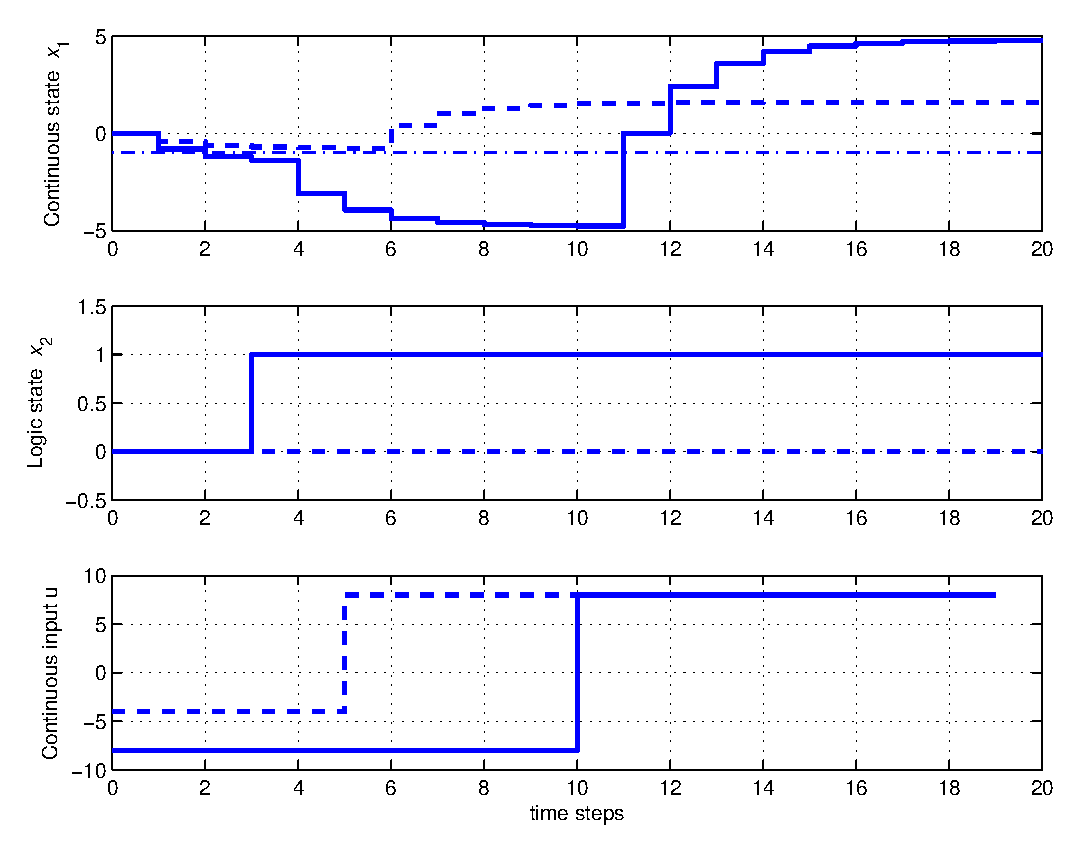
\includegraphics[width=.9\hsize]{switch3-OLsim.eps}}
   \caption{Open-loop simulation of system~(\ref{switch3}) for different
   input excitations}
   \label{ex:switch3-OLsim}
\end{figure}


\section{Discrete Hybrid Automata}
\label{sect::DHA}
As shown in Fig.~\ref{fig:dha}, a {\em discrete hybrid automaton} (DHA)
is formed by generating the mode
$i(t)$ of a switched affine system through a {\em mode selector}
function that depends on (1) the discrete state of a {\em finite state
machine}, (2) {\em discrete events}
generated by the continuous variables
of the switched affine system exceeding given linear thresholds (the guardlines),
(3) exogenous discrete inputs, and (4) time events~\cite{TB04a}.
We will detail each of the four blocks in the next sections.

\begin{figure}[t]
%$x_c(t)$\\[3em]
%$u_c(t)$\\[3em]
%$x_\ell(t)$\\[3em]
%$i(t)$\\[3em]
%$i(t-1)$\\[3em]
%$u_\ell(t)$\\[3em]
%$\delta_e(t)$
\psfrag{SAS}{SAS}
\psfrag{Automaton}{Automaton}
\psfrag{Event}{Event}
\psfrag{Generator}{Generator}
\psfrag{Mode}{Mode}
\psfrag{Selector}{Selector}
\psfrag{Clock}{Clock}
\psfrag{d}{{\footnotesize $~z^{-1}$}}
\psfrag{Switched}{Switched}
\psfrag{AS}{Affine System}
\begin{center}
\includegraphics[width=.7\columnwidth]{dtHS}%Original from HYSDEL paper: {redmodel}
\end{center}
\caption{A discrete hybrid automaton
(DHA) is the connection of a finite state machine (FSM) and a
switched affine system (SAS), through a mode selector (MS) and an
event generator (EG). The output signals are omitted for
clarity}
\label{fig:dha}
\end{figure}

\subsection{Switched Affine System (SAS)}
\label{sec:SAS}
A switched affine
system is a collection of affine systems:
\begin{subequations} \label{eq:sas}
\begin{eqnarray}
    x_c(t+1) &=& A_{i(t)}x_c(t) + B_{i(t)}u_c(t) + f_{i(t)},\label{eq:sas-x}\\
    y_c(t) &=& C_{i(t)}x_c(t) + D_{i(t)}u_c(t) + g_{i(t)},\label{eq:sas-y}
\end{eqnarray}
\end{subequations}
where $t\in \TT$ is the time indicator, $x_c \in \rr^{n_c}$ is the
continuous state vector, $u_c \in \rr^{m_c}$ is the exogenous
continuous input vector,
$y_c\in\rr^{p_c}$ is the
continuous output vector,
$\{A_{i},B_{i},f_{i},C_{i},D_{i},g_{i}\}_{i\in\II}$ is a
collection of matrices of suitable dimensions,
and the mode $i(t) \in \II\eqdef\{1,\ldots,s\}$
is an input signal that determines the affine state update
dynamics at time $t$. %We denote by $\sharp\II = s$ the number of elements in $\II$.
A SAS of the form~(\ref{eq:sas}) preserves the value of the state
when a mode switch occurs, however it is possible to implement reset
maps on a SAS as %we will show later in this section.
shown in~\cite{TB04a}.

\subsection{Event Generator (EG)}
\label{sec:eventgenerator}
An event generator is an object that generates a binary vector
$\delta_e(t)\in\{0,1\}^{n_e}$ of {\em event conditions} according
to the satisfaction of a linear (or affine) condition.

Let $h: \rr^{n_c} \times \rr^{n_c} \times \TT
\rightarrow \bol^{n_e}$ be a vector function defined as
\[
    h^i(x_c,u_c,t) =\left\{\ba{rll}
    1 & \mbox{if} & (A^{i})'x_c + (B^{i})'u_c+C^it+D^i \leq 0\\
    0 & \mbox{if} & (A^{i})'x_c + (B^{i})'u_c+C^it+D^i > 0
    \ea\right.
\]
where $^i$ denotes the $i$th component of a vector
or the $i$th row of a matrix, and $A$, $B$, $C$, $D$ are
constant matrices of suitable dimensions.
Then, events are defined as
\begin{equation}
\label{eq:eventgenerator}
    \delta_e(t)= h(x_c(t),u_c(t),t)
\end{equation}
In particular, {\em state events} are modeled as
$[\delta_e(t) = 1] \leftrightarrow [a'x_c(t)\leq b]$, while
{\em time events} are modeled as: $[\delta_e(t) = 1]
\leftrightarrow [tT_s \geq \tau_0]$, where $T_s$ is the sampling time and
$\tau_0$ is a given time.  In case time is explicitly involved
in~(\ref{eq:eventgenerator}), we can add the time as an additional
continuous and autonomous state variable $\tau$,
where $\tau(t+1)= \tau(t) + T_s$, so that the hybrid model
remains time-invariant.


\subsection{Boolean Algebra}
\label{sec:logic}
Before dealing in detail with the other blocks constituting the DHA
and introduce further notation, we recall here some basic
definitions of Boolean algebra\footnote{A more comprehensive treatment of Boolean calculus
can be found in digital circuit design texts, e.g.~\cite{Chr97,Hay93}.
For a rigorous exposition see e.g.~\cite{Men64}.}.

A variable $\delta$ is a Boolean variable if $\delta\in \{0,1\}$, where
``$\delta=0$'' means something is false, ``$\delta=1$'' that is true.
A Boolean expression is obtained by combining Boolean variables
through the logic operators $\lnot$
(not), $\OR$ (or), $\ANd$ (and), $\leftarrow$ (implied by),
$\rightarrow$ (implies), and $\leftrightarrow$ (iff).
A Boolean function $f:\{0,1\}^{n-1}\mapsto\{0,1\}$
is used to define a Boolean variable $\delta_n$ as
a logic function of other variables $\delta_1,\ldots,\delta_{n-1}$:
\begin{equation}
    \delta_n = f(\delta_1, \delta_2, \ldots, \delta_{n-1})
    \label{eq.ff}
\end{equation}
Given $n$ Boolean variables $\delta_1$, \ldots, $\delta_n$,
a Boolean formula $F$ defines a relation
\begin{equation}
    F(\delta_1, \ldots, \delta_n)
    \label{eq.F}
\end{equation}
that must hold true. Every Boolean formula $F(\delta_1,\delta_2,\ldots,\delta_n)$
can be rewritten in the conjunctive normal form (CNF)
\beqar
    \mbox{(CNF)}&&\bigwedge_{j=1}^m\left(\bigvee_{i\in P_j}\delta_i
  \bigvee_{i\in N_j}\NOT \delta_i\right)
\label{eq:CNF}\\
&&N_j,P_j \subseteq
\{1,\ldots,n\},~\forall j=1,\ldots,m.\nonumber
\eeqar

As mentioned in Section~\ref{sec:binary}, often will use
the term binary variable and Boolean variable without distinction.
An improper arithmetic operation over Boolean variables should be understood
as an arithmetic operation over corresponding binary variables and,
vice versa, an improper Boolean function of binary variables should be
interpreted as the same function over the corresponding Boolean variables.
Therefore, from now on we will call ``binary'' variables both 0-1 variables
and Boolean variables.

\subsection{Finite State Machine (\emph{FSM})}
A finite state machine\footnote{In this notes we will only refer to synchronous
finite state machines, where the transitions may happen only at
sampling times. The adjective synchronous will be omitted for
brevity.} (or automaton) is a discrete dynamic process that
evolves according to a Boolean state update function:
\begin{subequations}
\begin{equation}
    x_\ell(t+1) = f_\ell(x_\ell(t),u_\ell(t),\delta_e(t)){\rm ,}
\end{equation}
where $x_\ell \in \bol^{n_\ell}$ is the binary state, $u_\ell \in
\bol^{m_\ell}$ is the exogenous binary input, $\delta_e(t)$ is the
endogenous binary input coming from the EG, and $f_\ell:
\bol^{n_\ell} \times \bol^{m_\ell} \times \{0,1\}^{n_e}
 \rightarrow \bol^{n_\ell}$ is a deterministic Boolean function.

A FSM can be conveniently
represented using an oriented graph. A FSM may also have
an associated binary output
\begin{equation}
    y_\ell(t) = g_\ell(x_\ell(t),u_\ell(t),\delta_e(t)){\rm ,}
\end{equation}
\end{subequations}
where $y_\ell \in \bol^{p_\ell}$
and $g_\ell:\bol^{n_\ell}\times\bol^{m_\ell}\times\{0,1\}^{n_e}\mapsto \bol^{p_\ell}$.

\example{ex:automa}{
\begin{figure}[t]
  \centering \psfrag{a}[r][r]{$\NOT \delta_3$}
  \psfrag{b}[l][l]{$\delta_1 \ANd u_{\ell2}$}
  \psfrag{c}[l][l]{$\delta_1 \ANd \NOT u_{\ell2}$}
  \psfrag{d}[c][c]{$\delta_2$}
  \psfrag{e}[c][c]{$ \delta_3 \ANd u_{\ell1}$}
  \psfrag{f}[c][c]{$\NOT\delta_1$}
  \psfrag{h}[c][c]{$\NOT u_{\ell1} \ANd \delta_3$}
  \psfrag{i}[c][c]{$\NOT\delta_2$}
  \psfrag{R}[c][c][.8]{\small{\sf Red}}
  \psfrag{G}[c][c][.8]{\small{\sf Green}} \psfrag{B}[c][c][.8]{\small{\sf Blue}}
  \includegraphics[width=.6\hsize]{fsm}
  \caption{Example of finite state machine}
  \label{fig:fsm}
\end{figure}
Figure~\ref{fig:fsm} shows a finite state machine where
$u_\ell=[u_{\ell1}~u_{\ell2}]^T$ is the input vector, and $\delta = [\delta_1
\ldots \delta_3]^T$ is a vector of signals coming from the event
generator. The Boolean state update function (also called {\em state transition
  function}) is:
\begin{equation}
    x_\ell(t+1) = \left\{
    \begin{array}{l}
    {\sf Red} ~{\rm if}~((x_\ell(t) = {\sf Green}) \ANd \NOT
    \delta_3) \OR \\
    ~~~~~((x_\ell(t) = {\sf Red}) \ANd \NOT \delta_1), \\
    {\sf Green} ~ {\rm if} ~ ((x_\ell(t) = {\sf Red}) \ANd
    \delta_1 \ANd u_{\ell2})\OR \\
    ~~~~~((x_\ell(t) = {\sf Blue}) \ANd \delta_2) \OR \\
    ~~~~~((x_\ell(t) = {\sf Green}) \ANd \NOT u_{\ell1} \ANd \delta_3), \\
    {\sf Blue} ~ {\rm if} ~ ((x_\ell(t) = {\sf Red}) \ANd \delta_1 \ANd
    \NOT u_{\ell2}) \OR \\
    ~~~~~((x_\ell(t) = {\sf Green}) \ANd (\delta_3 \ANd u_{\ell1})) \OR\\
    ~~~~~((x_\ell(t) = {\sf Blue}) \ANd \NOT \delta_2))\mbox{\rm .} \\
    \end{array}
    \right.
    \label{eq:exauto}
\end{equation}
By associating a binary vector $x_\ell = \smallmat{x_{\ell1}\\x_{\ell2}}$ to each state (${\sf Red} =
\smallmat{0\\0}$, ${\sf Green} = \smallmat{0\\1}$, and ${\sf Blue}
= \smallmat{1\\0}$), one can rewrite~(\ref{eq:exauto}) as:
\begin{eqnarray*}
x_{\ell1}(t+1)     &=&
            (\NOT x_{\ell1} \ANd \NOT x_{\ell2} \ANd  \delta_1 \ANd \NOT
            u_{\ell2} ) \OR \\
            && ( x_{\ell1} \ANd \NOT \delta_2 ) \OR
             ( x_{\ell2} \ANd  \delta_3 \ANd  u_{\ell1} ),\\
x_{\ell2}(t+1)     &=&
             (\NOT x_{\ell1} \ANd \NOT x_{\ell2} \ANd  \delta_1 \ANd  u_{\ell2}
            ) \OR \\
            && ( x_{\ell1} \ANd  \delta_2 ) \OR
             ( x_{\ell2} \ANd  \delta_3 \ANd \NOT u_{\ell1} ),
\end{eqnarray*}
where the time index $(t)$ has been omitted for brevity.
}\cvd

Since the Boolean state update function is
deterministic, for each state the conditions associated
with all the outgoing arcs are mutually exclusive.

\subsection{Mode Selector}
In a DHA, the dynamic mode $i(t)\in\II=\{1,\ldots,s\}$ of the SAS is
a function of the binary state $x_\ell(t)$, the  binary input $u_\ell(t)$, and the events
$\delta_e(t)$. With a slight abuse of notation, let us indicate the mode
$i(t)$ through its binary encoding, $i(t)\in\{0,1\}^{n_s}$ where
$n_s=\lceil \log_2 s\rceil$, so that $i(t)$ can be treated as a vector
of Boolean variables\footnote{Any discrete variable
$\alpha \in \{\alpha_1,\ldots,\alpha_j\}$ admits a Boolean
encoding $a \in \bol^{d(j)}$, where $d(j)$ is the number of bits
used to represent $\alpha_1$, \ldots, $\alpha_j$.
For example, $\alpha\in\{0,1,2\}$ may be encoded as
$a\in\{0,1\}^2$ by associating $\smallmat{0\\0}\rightarrow 0$,
$\smallmat{0\\1}\rightarrow 1$, $\smallmat{1\\0}\rightarrow 2$.}.
Then, we define the {\em mode selector} by the
Boolean function $f_{\rm M}: \bol^{n_\ell} \times \bol^{m_\ell} \times
\bol^{n_e} \rightarrow \{0,1\}^{n_s}$. The  output of
this function
\begin{equation}
  i(t)=\mu(x_\ell(t),u_\ell(t),\delta_e(t))
    \label{eq:MS}
\end{equation}
is called the {\em active mode} of the DHA at time $t$.
We say that a {\em mode switch} occurs at
step $t$ if $i(t)\neq i(t-1)$. Note that, in contrast to
continuous-time hybrid models where switches can occur at any time,
in our discrete-time setting a mode switch can only occur at sampling
instants.


\subsection{DHA Trajectories}
\label{sec:dha-trajectories}
For a given initial condition $\smallmat{x_c(0)\\x_\ell(0)}\in\rr^{n_c}\times\bol^{n_\ell}$,
and inputs $\smallmat{u_c(t)\\u_\ell(t)}\in\rr^{m_c}\times\bol^{m_\ell}$,
$t\in\TT$, the state $x(t)$ of the system is recursively computed as
follows for all $t\in\TT$:
 \begin{enumerate}
 \item Initialization: $x(0) = \smallmat{x_c(0)\\x_\ell(0)}$;
 \item Recursion: given $x(t) = \smallmat{x_c(t)\\x_\ell(t)}$
 and $u(t) = \smallmat{u_c(t)\\u_\ell(t)}$, evaluate $x(t+1)$
 and $y(t) = \smallmat{y_c(t)\\y_\ell(t)}$ in the following order:
 \begin{subequations}
 \beqar
 \delta_e(t) &=& h(x_c(t),u_c(t),t)\\
 i(t) &=& \mu(x_\ell(t),u_\ell(t),\delta_e(t))\\
 y_c(t) &=& C_{i(t)}x_c(t) + D_{i(t)}u_c(t) + g_{i(t)}\\
 y_\ell(t) &=&  g_\ell(x_\ell(t),u_\ell(t),\delta_e(t))\\
 x_c(t+1) &=& A_{i(t)}x_c(t) + B_{i(t)}u_c(t) + f_{i(t)}\\
 x_\ell(t+1) &=&  f_\ell(x_\ell(t),u_\ell(t),\delta_e(t))
 \eeqar
 \end{subequations}
 \label{eq:DHA}%
 \end{enumerate}
A definition of well-posedness of DHA can be given similarly to
Definition~\ref{def:well-posedness} by requiring that the successor
states $x_c(t+1)$, $x_\ell(t+1)$ and the outputs
$y_c(t)$, $y_\ell(t)$ are uniquely defined functions of $x_c(t)$, $x_\ell(t)$,
$u_c(t)$, $u_\ell(t)$ defined by the DHA equations~(\ref{eq:DHA}).

%Definition~\ref{def:well-posed} will be used for other types of hybrid
%models that we will introduce later.  In general a hybrid model may
%not be well-posed, either because the trajectories stop after a finite
%time (for instance, the state vector leaves the set
%$\XX_c\times\bol^{n_\ell}$) or because of non-determinism (the successor
%$x_c'(t)$, $x_\ell'(t)$ may be multiply defined). Note that
%trajectories of DHA are deterministic.

DHA can be considered as a subclass of {\em hybrid automata}
(HA)~\cite{ACHH93}. The main difference is in the time model: DHA
are based on discrete time, HA on continuous time.
Moreover DHA models do not allow
instantaneous transitions, and are deterministic, opposed to HA
where any enabled transition may occur in zero time. This has two
consequences (i) DHA do not admit live-locks (infinite switches in
zero time), (ii) DHA do not admit Zeno behaviors (infinite
switches in finite time). Finally in DHA models, guards, reset
maps and continuous dynamics are limited to linear (or affine)
functions.
%However, working with discrete-time models enables us solving
%complex constrained optimal control problems.


\section{Logic and Mixed-Integer Inequalities}
\label{sec:MIP}
%\annote{Fare un cappello, motivando perche' si vuole tradurre
%in inequalities e citando vecchi risultati su LOGIC->MIP}
Despite the fact that DHA are rich of expressiveness and
are therefore quite suitable for modeling and simulating
hybrid dynamical systems, they are not directly
suitable for solving optimal control problems, because of
their heterogeneous discrete and continuous nature.
In this section we want to describe how DHA can be translated
into different hybrid models that are more suitable
for optimization. We highlight the main techniques of the translation
process, by generalizing several results that appeared in the
literature~\cite{Glo75,RG91,Wil93,MLM94,CH99,BM99,%
Hurl01,CPS90,TM99,Wil77,NeWo88}.

\subsection{Transformation of Boolean Relations}
\label{sec:Boolean}

Boolean formulas can be equivalently represented as integer
linear inequalities. For instance, $\delta_1\lor \delta_2=1$ is
equivalent to $\delta_1+\delta_2\geq 1$~\cite{Wil93}. Some recurrent
equivalences are reported in Table~\ref{tab:Logic-MIP}.

\begin{table}[t]
\begin{center} \hspace*{-0.5cm}
{\footnotesize\bf
\begin{tabular}{|c|c|c|} \hline\hline
      relation & Boolean & linear constraints\\\hline\hline
AND & $\delta_1 \wedge \delta_2$ & $\delta_1=1$, $\delta_2=1$ or $\delta_1+\delta_2\geq 2$\\\hline
% d1 OR d2
OR & $\delta_1 \vee X_2 $ & $\delta_1 + \delta_2 \geq 1$ \\
\hline
% NOT d1
NOT & $\NOT \delta_1$ & $\delta_1=0$\\\hline
% d1 XOR d2
XOR & $\delta_1 \oplus \delta_2 $ &
$\delta_1 + \delta_2 = 1$\\
\hline
% d1 IMPLY d2
IMPLY & $\delta_1 \rightarrow \delta_2 $ & $\delta_1 - \delta_2
\leq 0$ \\\hline
% d1 IFF d2
IFF  & $\delta_1 \leftrightarrow \delta_2 $ & $\delta_1 -
\delta_2 = 0$\\\hline
%d3=d1 AND d2
ASSIGNMENT  &         & $\delta_1+(1-\delta_3)\geq 1$ \\
  $\delta_3 =\delta_1\wedge \delta_2$    &
  $\delta_3\leftrightarrow \delta_1\wedge \delta_2$& $\delta_2 +(1- \delta_3)   \geq 1$ \\
  &  &   $(1-\delta_1) + (1-\delta_2)+ \delta_3 \geq 1$
\\\hline\hline
\end{tabular}
}
\end{center}
\caption{Basic conversion of Boolean relations into
mixed-integer inequalities. Relations involving the inverted
literals $\NOT \delta$ can be obtained by substituting $(1-\delta)$ for $\delta$
in the corresponding inequalities. More conversions are reported
in~\cite{Mig02}, or can be derived by~(\ref{eq:CNF})--(\ref{eq:CNFineq})}
\label{tab:Logic-MIP}
\end{table}

In general, for every Boolean formula $F(\delta_1,\delta_2,\ldots,\delta_n)$
there exists a polyhedral set $P$ such that a set of binary values
$\{\delta_1,\delta_2,\ldots,\delta_n\}$ satisfies the Boolean
formula $F$ if and only if $\delta=[\delta_1\ \delta_2\ \ldots\
\delta_n]'\in P$.

Given a formula $F$, one way of constructing one of such polyhedra $P$ is to
rewrite $F$ in the conjunctive normal form~(\ref{eq:CNF}), and then simply
define $P$ as
\begin{equation}
   P=\left\{\delta\in\{0,1\}^n:~
  \ba{ll}
    1\leq \sum_{i\in P_1}\delta_i&+\sum_{i\in N_1}(1-\delta_i) \\
     &\vdots\\
    1\leq \sum_{i\in P_m}\delta_i&+\sum_{i\in N_m}(1-\delta_i)
  \ea\right\}
    \label{eq:CNFineq}
\end{equation}

The smallest polyhedron $P$ associated with formula $F$ has the
following geometric interpretation:
Assume to list all the 0-1 combinations of $\delta_i$'s
satisfying $F$ (namely, to generate the truth table of $F$), and
think each combination as an $n$-dimensional binary vector in $\rr^n$,
then $P$ is the convex hull of such vectors~\cite{CH99,Hoo00,MBM99a}.
For methods to compute convex hulls, we refer the reader to~\cite{Fuk97}.

\subsection{Translating DHA Components into Linear Mixed-Integer Relations}
\label{sect.cli}
Events of the form~(\ref{eq:eventgenerator}) can
be expressed equivalently as
\begin{subequations} \label{eq:threshold-ineq}
\begin{align}
  h^i(x_c(t),u_c(t),t)&\leq M^i(1-\delta_e^i),\label{eq:ti1}\\
  h^i(x_c(t),u_c(t),t)&> m^i\delta^i_e, \quad \qquad
  i=1,\ldots,n_e,\label{eq:ti2}
\end{align}
where $M^i$, $m^i$ are upper and lower bounds,
respectively, on $h^i(x_c(t),u_c(t),t)$.
As we have pointed out in Section~\ref{sect:dPWA}, from a
computational viewpoint it is convenient to avoid
strict inequalities. As suggested in~\cite{Wil93},
we modify the strict inequality~(\ref{eq:ti2}) into
\begin{equation}
  h^i(x_c(t),u_c(t),t) \geq\epsilon+(m^i-\epsilon)\delta^i_e
  \label{eq:ti3}
\end{equation}
where $\epsilon$ is a small positive scalar (e.g., the machine
precision). Clearly, as for the case of discontinuous PWA
discussed in Section~\ref{sect:dPWA},
Equations~(\ref{eq:threshold-ineq}) or (\ref{eq:eventgenerator})
are equivalent to~(\ref{eq:ti3}) only for $h^i(x_c(t),u_c(t),t)\leq 0$
and $h^i(x_c(t),u_c(t),t)\geq\epsilon$.
\end{subequations}

Regarding switched affine dynamics, we first rewrite
the state-update equation~(\ref{eq:sas-x}) as the following combination of
affine terms and \emph{if-then-else} conditions:
\begin{subequations}
\label{eq:z-transform}
\begin{align}
     z_1(t) &= \left\{
  \begin{array}{ll}
    A_1 x_c(t) + B_1 u_c(t) + f_1, & {\rm if~}  (i(t) = 1), \\
    0, & {\rm otherwise},
  \end{array} \right. \label{eq:z-transform-a}\\
%
   & \ \ \vdots \nonumber \\
%
    z_s(t) &= \left\{
  \begin{array}{ll}
    A_s x_c(t) + B_s u_c(t) + f_s, & {\rm if~}  (i(t) = s), \\
    0, & {\rm otherwise}, \\
  \end{array} \right.   \label{eq:z-transform-b}\\
%
  x_c(t+1) &= \sum_{i=1}^s z_i(t), \label{eq:z-transform-c}
\end{align}
\end{subequations}
where $z_i(t)\in \rr ^{n_c},i = 1,\ldots,s$. The output
equation~(\ref{eq:sas-y}) admits a similar transformation.

A generic if-then-else construct of the form
\begin{equation}
  \mbox{IF}\ \delta\ \mbox{THEN}\ z=a_1'x+b_1'u+f_1\ \mbox{ELSE}\
  z=a_2'x+b_2'u +f_2,
    \label{eq:if-then-else}
\end{equation}
where $\delta \in \bol$, $z \in \rr$, $x \in
\rr^n$, $u \in \rr^m$, and $a_1,b_1,f_1,a_2,b_2,f_2$
are constants of suitable dimensions, can be translated into~\cite{BTM01a}
\begin{subequations}  \label{eq:if-ineq}
    \beqar
          (m_2-M_1)\delta+z&\leq &a_2'x+b_2'u+f_2, \\
          (m_1-M_2)\delta-z&\leq &-a_2'x-b_2'u-f_2,\\
          (m_1-M_2)(1-\delta)+z&\leq &a_1'x+b_1'u+f_1,\\
          (m_2-M_1)(1-\delta)-z&\leq &-a_1'x-b_1'u-f_1,
    \eeqar%
\end{subequations}
where $M_i$, $m_i$ are upper and lower bounds on
$a_ix+b_iu+f_i$, $i=1,2$. Note that
when $a_2=0$, $b_2=0$, $f_2=0$, relations
(\ref{eq:if-then-else})--(\ref{eq:if-ineq}) model
the real product $z=\delta \cdot (a_1'x+b_1'u+f)$ described
in~\cite{Wil93}.

Finally, the mode selector function and binary state-update function
of the automaton are Boolean functions that can be translated into integer
linear inequalities as described in Section~\ref{sec:Boolean}.
The idea of transforming a
well-posed FSM into a set of Boolean equalities was also presented
in~\cite{PB97} where the authors performed model checking using (mixed)
integer optimization on an equivalent set of integer inequalities.

\section{Mixed Logical Dynamical Systems}
\label{sec:MLD}
Given a DHA representation of a hybrid process, by following
the techniques described in the previous section for converting logical relations
into inequalities we obtain an equivalent representation of the DHA as
a \emph{mixed logical dynamical} (MLD) system~\cite{BM99}.

An MLD system is described by the following
relations:
\begin{subequations}\label{eq:MLD}%
\begin{align}
    x(t+1)&=\Aa x(t)+\BB_{1}u(t)+\BB_{2}\delta(t)+\BB_{3}z(t)+\BB_5,\label{eq:MLD-a}\\
    y(t)&=\Cc x(t)+\DD_{1}u(t)+\DD_{2}\delta(t)+\DD_{3}z(t)+\DD_5,\label{eq:MLD-b}\\
    &\EE_{2}\delta(t)+\EE_{3}z(t)\leq
    \EE_{1}u(t)+\EE_{4}x(t)+\EE_{5},\label{eq:MLD-c}
    %&\overline\EE_{2}\delta(t)+\overline\EE_{3}z(t)=\overline\EE_{1}u(t)+
    %\overline\EE_{4}x(t)+\overline\EE_{5}.\label{eq:MLD-d}\\
    %&\tilde \EE_{2}\delta(t)+\tilde \EE_{3}z(t)<\tilde \EE_{1}u(t)+\tilde \EE_{4}x(t)+\tilde \EE_{5}.\label{eq:MLD-e}
\end{align}%
\end{subequations}
\noindent where $x\in\rr^{n_c}\times\{0,1\}^{n_\ell}$ is a vector of
continuous and binary states, $u\in \rr^{m_c}\times\{0,1\}^{m_\ell}$ are
the inputs, $y\in \rr^{p_c}\times\{0,1\}^{p_\ell}$ the outputs,
$\delta\in\{0,1\}^{r_\ell}$ are auxiliary binary variables,
$z\in\rr^{r_c}$ are continuous auxiliary variables,
and $\Aa$, $\BB_1$, $\BB_2$,
$\BB_3$, $\Cc$, $\DD_1$, $\DD_2$, $\DD_3$, $\EE_1$,\ldots,$\EE_5$
%$\tilde \EE_1$,\ldots,$\tilde \EE_5$
%$\overline\EE_1$,\ldots,$\overline\EE_5$
are matrices of suitable
dimensions. Given the current state $x(t)$ and input $u(t)$, the
time-evolution of~(\ref{eq:MLD}) is determined by finding a feasible
value for $\delta(t)$ and $z(t)$ satisfying~(\ref{eq:MLD-c}), and then by computing
$x(t+1)$ and $y(t)$ from~(\ref{eq:MLD-a})--(\ref{eq:MLD-b}).

As MLD models consist of a collection of linear difference
equations involving both real and binary variables and a set of
linear inequality constraints, they are model representations
of hybrid systems that can be easily used in optimization
algorithms, as will be described in Chapter~\ref{optimal_control}.

A definition of well-posedness of the MLD system~(\ref{eq:MLD})
can be given similarly to Definition~\ref{def:well-posedness} by requiring
that for all $x(t)$ and $u(t)$ within a given bounded set the pair
of variables $\delta(t)$, $z(t)$ satisfying~(\ref{eq:MLD-c}) is unique,
so that the successor state $x(t+1)$ and output
$y(t)$ are also uniquely defined functions of $x(t)$, $u(t)$
through~(\ref{eq:MLD-a})--(\ref{eq:MLD-b})\footnote{For a more general definition
of well-posedness of MLD systems see~\cite{BM99}.}.

The well-posedness assumption is usually guaranteed by
the procedure described in Section~\ref{sec:logic}
used to generate the linear
inequalities~(\ref{eq:MLD-c}). Nevertheless, a numerical test for
well-posedness is reported in~\cite[Appendix~1]{BM99}.

Note that the constraints~(\ref{eq:MLD-c}) allow one
to specify additional linear constraints
on continuous variables (e.g., constraints over
physical variables of the system), and logical constraints over
Boolean variables. The ability to include constraints,
constraint prioritization, and heuristics adds to the
expressiveness and generality of the MLD framework.
Note also that
despite the fact that the description (\ref{eq:MLD}) seems to be
linear, clearly the nonlinearity is concentrated
in the integrality constraints over binary variables.

\example{ex:BM99}{
Consider the following simple switched linear system~\cite{BM99}
\begin{equation}
    x(t+1)=\left\{\ba{rcl}
           0.8x(t)+u(t) & \mbox{if} & x(t)\geq 0\\
           -0.8 x(t)+u(t) & \mbox{if} & x(t) < 0
           \ea\right.
    \label{MIPC2}
\end{equation}
where $x(t)\in[-10,10]$, and $u(t)\in[-1,1]$. The condition $x(t)\geq 0$
can be associated to an event variable $\delta(t)\in\{0,1\}$ defined
as
\begin{equation}
    \left[\delta(t)=1\right]\ \leftrightarrow\ \left[x(t)\geq 0\right].
    \label{MIPC2-cond}
\end{equation}
By using the transformations~(\ref{eq:ti1})--(\ref{eq:ti3}),
equation~(\ref{MIPC2-cond}) can be expressed by the inequalities
\begin{subequations}
\beqar
    -m\delta(t) & \leq & x(t)-m\\
    -(M+\epsilon)\delta(t) & \leq & -x(t)-\epsilon
\eeqar
\label{eq:simple-delta}%
\end{subequations}
where $M=-m=10$, and $\epsilon$ is an arbitrarily small positive scalar. Then~(\ref{MIPC2})
can be rewritten as
\begin{equation}
    x(t+1)=1.6\delta(t)x(t)-0.8x(t)+u(t).
    \label{MIPC2-2}
\end{equation}
By defining a new variable $z(t)=\delta(t)x(t)$ which,
by~(\ref{eq:if-then-else})--(\ref{eq:if-ineq})
can be expressed as
\begin{subequations}
\beqar
    z(t)&\leq &M\delta(t)\\
    z(t)&\geq &m\delta(t)\\
    z(t)&\leq &x(t)-m(1-\delta(t))\\
    z(t)&\geq &x(t)-M(1-\delta(t)),
\eeqar
\label{eq:simple-zeta}
\end{subequations}
the evolution of system~(\ref{MIPC2}) is ruled by the linear equation
\begin{equation}
   x(t+1)=1.6z(t)-0.8x(t)+u(t)
   \label{eq:simple-stateupdate}
\end{equation}
subject to the linear constraints~(\ref{eq:simple-delta})
and~(\ref{eq:simple-zeta}). Therefore, the MLD equivalent representation
of~(\ref{MIPC2}) for $x\in[-10,-\epsilon]\cup[0,10]$ and $u\in[-1,1]$
is given by collecting Equations~(\ref{eq:simple-stateupdate}),~(\ref{eq:simple-delta})
and ~(\ref{eq:simple-zeta}).
} % \end{example}

Finally we recall that the MLD model
is similar to the model presented in~\cite{DSP97} for verification of
safety properties as they both aim at translating a hybrid system in a
set of mixed integer linear equalities and inequalities using similar
techniques.

\section{Model Equivalences}
In the previous chapters we have presented three different classes of
discrete-time hybrid models: PWA systems, DHA, and MLD systems.
For what we described in Section~\ref{sec:logic}, under the assumption
that the set of valid states and inputs is bounded, DHA systems can always be
equivalently described as MLD systems. Also, a PWA system is a special case
of a DHA whose threshold events and mode selector function are defined by the
PWA partition. Therefore, a PWA system with bounded partition $\XX$
can always be described as an MLD system
(an efficient way of modeling PWA systems in MLD form is reported in~\cite{BM99}).

The converse result, namely that MLD systems (and therefore DHA) can be represented as
PWA systems, is less obvious. Under the condition that the
MLD system is well-posed, this result was proved in \cite{BFM00}.
A slightly different and more general proof is reported in~\cite{Bem04a},
where the author also provides efficient MLD to PWA translation algorithms.
A different algorithm for obtaining a PWA representation of
a DHA is reported in~\cite{GTM03}.

Such equivalence results are of interest because
DHA are most suitable in the modeling phase, but MLD are most suitable for
solving open-loop finite-time optimal control problems, and PWA are most suitable
for solving finite-time optimal control problems in state-feedback form, as will
be described in Chapter~\ref{optimal_control}.

The fact that PWA systems are equivalent to interconnections of linear
systems and finite automata was also pointed out by Sontag~\cite{Son96}.
In~\cite{HDB01a} the authors proved the equivalence of discrete-time PWA/MLD
systems with other classes of discrete-time hybrid systems (possibly under
some hypothesis) such as linear complementarity (LC)
systems~\cite{Hee99,vdSS98,HSW00}, extended linear complementarity
(ELC) systems~\cite{dSdM98}, and max-min-plus-scaling (MMPS)
systems~\cite{dSvdB01}.


\section{The \hysdel{} Modeling Language}
A modeling language was proposed in~\cite{TB04a}
to describe DHA models, called HYbrid
System DEscription Language (\hysdel{}).  The \hysdel{}
description of a DHA is an abstract modeling step. The associated \hysdel{}
compiler then translates the description into several computational
models, in particular into a MLD using the technique presented in
Section~\ref{sec:MIP}, and PWA form using either the
approach of~\cite{GTM03} or the approach of~\cite{Bem04a}.
\hysdel{} can generate also a simulator that runs as a function in
Matlab. The \hysdel{} compiler is available at
\url{http://control.ee.ethz.ch/~hybrid/hysdel} and is supported
by the Hybrid Toolbox (\url{http://www.dii.unisi.it/hybrid/toolbox})
and by the Multiparametric Toolbox (\url{http://control.ee.ethz.ch/~mpt}).

In this section we show how a DHA system can be modeled in
\hysdel{} by illustrating the \hysdel{} description of the following
DHA system:
%(\ref{eq:systemreset}).
\begin{subequations}  \label{eq:systemreset}
\begin{align}
  \mbox{\rm SAS:~} &
  x_c'(t) = \left\{
  \begin{array}{lcl}
    x_c(t) + u_c(t) - 1, & {\rm if } & i(t)=1, \\
    2x_c(t), & {\rm if } & i(t)=2, \\
    2, & {\rm if} & i(t)=3,
  \end{array}
  \right. \\
%
  \mbox{\rm EG:~} &
  \left\{
    \begin{array}{l}
    \delta_e(t) = [x_c(t) \ge 0], \\
    \delta_f(t) = [x_c(t) + u_c(t) - 1 \ge 0],
  \end{array}
  \right.
  \\
%
  \mbox{\rm MS:~} &
  i(t) = \left\{
  \begin{array}{lcl}
    1, & {\rm if } & \smallmat{\delta_e(t)\\\delta_f(t)} = \smallmat{0\\0},\\
    2, & {\rm if } & \delta_e(t) = 1, \\
    3, & {\rm if } & \smallmat{\delta_e(t)\\\delta_f(t)} = \smallmat{0\\1}.
  \end{array}
  \right.
\end{align}
\end{subequations}

\begin{table}[t]
{  \hysdeltext
\begin{verbatim}
SYSTEM sample {
INTERFACE {
  STATE {
    REAL xr [-10, 10]; }
  INPUT {
    REAL ur [-2, 2]; }
}
IMPLEMENTATION {
  AUX {
    REAL z1, z2, z3;
    BOOL de, df, d1, d2, d3; }
  AD {
    de = xr >= 0;
    df = xr + ur - 1 >= 0; }
  LOGIC {
    d1 = ~de & ~df;
    d2 = de;
    d3 = ~de & df; }
  DA {
    z1 = {IF d1 THEN xr + ur - 1 };
    z2 = {IF d2 THEN 2 * xr };
    z3 = {IF (~de & df)  THEN 2 }; }
  CONTINUOUS {
    xr = z1 + z2 + z3; }
}}
\end{verbatim}
}

  \caption{Sample \hysdel{} list of system~(\ref{eq:systemreset})}
  \label{tab:hysdellist}
\end{table}

Consider the \hysdel{} list of Table~\ref{tab:hysdellist}. As any
\hysdel{} list, it is composed of two parts. The first one, called
\hs{INTERFACE}, contains the declaration of all variables and
parameters, so that it is possible to make the proper type checks. The
second part, \hs{IMPLEMENTATION}, is composed of specialized sections
where the relations among the variables are described. These sections
are described next.

\desc{\hs{AUX} Section} The \hysdel{} section \hs{AUX} contains the
declaration of the auxiliary variables used in the model. These variables
will become the $\delta$ and $z$ variables in the MLD model~(\ref{eq:MLD}).

\desc{\hs{AD} Section} The \hysdel{} section \hs{AD} allows one to define
Boolean variables from continuous ones, and is based exactly on the
same semantics of the event generator (EG) described earlier.  \hysdel{}
does not provide explicit access to the time instance, however this
limitation can be easily overcome as described in Section~\ref{sec:eventgenerator}.

\desc{\hs{LOGIC} Section} The section \hs{LOGIC} allows one to specify
arbitrary functions of Boolean variables: In particular the mode
selector is a Boolean function that can be modeled in this
section.

\desc{\hs{DA} Section} The \hysdel{} section \hs{DA} defines continuous
variables according to if-then-else conditions.
This section models part of the switched affine system (SAS), namely
the variables $z_i$ defined
in~(\ref{eq:z-transform-a})--(\ref{eq:z-transform-b}). Note that, as
the definition of \texttt{z3} suggests, \hysdel{} can handle compound logic
formulas in the \hs{DA} section, therefore there is no need to explicitly
define a Boolean variable for each mode.

\desc{\hs{CONTINUOUS} Section} The \hs{CONTINUOUS} section describes
the linear dynamics, expressed as difference equations. This section
models~(\ref{eq:z-transform-c}).

A \hysdel{} description may have additional sections that are not
part of the sample code of Table~\ref{tab:hysdellist}, that we describe
below. For examples and the detailed syntax we refer the interested reader
to~\cite{TBBHJM02}.

\desc{\hs{LINEAR} Section} \hysdel{} allows also one to define a continuous
variable as an affine function of continuous variables in the
\hs{LINEAR} section. This section, together with the \hs{CONTINUOUS}
and \hs{AD} sections allows more flexibility when modeling the SAS.
This extra flexibility allows algebraic loops that may render
undefined the trajectories of the model. The \hysdel{} compiler
integrates a semantic checker that is able to detect and report such
abnormal situations.

\desc{\hs{AUTOMATA} Section} The \hs{AUTOMATA} section specifies
the state transition equations of the finite state machine (FSM)
as a collection of Boolean functions
$x_{\ell i}'(t) = f_{{\rm B}i}(x_\ell(t),u_\ell(t),\delta_e(t))$, $i=1,\ldots,n_\ell$.

\desc{\hs{OUTPUT} Section} The \hs{OUTPUT} section allows one to
specify static linear and logic relations for the output vector
$y=\smallmat{y_c\\y_\ell}$.

Finally \hysdel{} allows one more section:

\desc{\hs{MUST} Section} This section
specifies arbitrary linear and logic constraints %Boolean formulas
on continuous and Boolean variables, and
therefore it allows for defining the sets $\XX_c$, $\bol^{n_\ell}$, $\rr^{m_c}$,
$\bol^{m_\ell}$, $\rr^{p_c}$, $\bol^{p_\ell}$ (more generally, the \hs{MUST} section
allows also mixed constraints on states, inputs, and outputs).

\hysdel{} allows generating MLD models in Matlab.
Thanks to the equivalences mentioned in the previous section,
such models can be immediately (and efficiently) translated
into PWA systems~\cite{Bem04a,GTM03}.

\begin{table}
{\hysdeltext
\begin{verbatim}
/* 2x2 PWA system */

SYSTEM pwa {

INTERFACE {
    STATE { REAL x1 [-5,5];
            REAL x2 [-5,5];
        }
    INPUT { REAL u [-1,1];
        }
    OUTPUT{ REAL y;
        }
    PARAMETER {
        REAL alpha = 60*pi/180;
        REAL C = cos(alpha);
        REAL S = sin(alpha);
        REAL MLD_epsilon = 1e-6;    }
    }

IMPLEMENTATION {
        AUX { REAL z1,z2;
              BOOL sign; }
        AD  { sign = x1<=0; }

        DA  { z1 = {IF sign THEN 0.8*(C*x1+S*x2)
                    ELSE 0.8*(C*x1-S*x2) };
              z2 = {IF sign THEN 0.8*(-S*x1+C*x2)
                    ELSE 0.8*(S*x1+C*x2) };  }

        CONTINUOUS { x1 = z1;
                     x2 = z2+u; }

        OUTPUT { y = x2;  }
      }
}
\end{verbatim}
}
\caption{HYSDEL model of the PWA system described in Example~\ref{ex:simple-example}}
\label{tab:HYSDEL-simple-example}
\end{table}

\example{ex:simple-example2}{Consider again the PWA system described
in Example~\ref{ex:simple-example}.
Assuming that $[-5,5]\times[-5,5]$ is the set of states $x(t)$
of interest, using \hysdel{} we describe~(\ref{switch}) as
described in Table~\ref{tab:HYSDEL-simple-example}
and obtain the equivalent MLD form
\[
    \hspace*{-.5cm}\ba{l}
    x(t+1)=\smallmat{1 &0 \\0 &1}z(t)+\smallmat{0\\1}u(t)\\
    y(t)=\smallmat{0 & 1}x(t)\\
    \smallmat{
    -5-\epsilon\\
     5\\
    c_1\\
    c_1\\
   -c_1\\
   -c_1\\
    c_1\\
    c_1\\
   -c_1\\
   -c_1}\delta(t)+\smallmat{
         0  &   0 \\
         0  &   0 \\
        -1  &   0 \\
         1  &   0 \\
        -1  &   0 \\
         1  &   0 \\
         0  &  -1 \\
         0  &   1 \\
         0  &  -1 \\
         0  &   1}z(t)\leq\smallmat{
      1& 0 \\
     -1& 0\\
     -0.4 &  -c_2 \\
      0.4 & c_2 \\
     -0.4 & c_2 \\
      0.4 & -c_2 \\
      c_2 & -0.4\\
     -c_2 &  0.4\\
     -c_2 & -0.4\\
      c_2 &  0.4}x(t)+\smallmat{
  -\epsilon\\
   5\\
  c_1\\
  c_1\\
                  0\\
                  0\\
  c_1\\
  c_1\\
                  0\\
                  0}.
    \ea
\]
where $c_1=4(\sqrt 3+1)$, $c_2=0.4\sqrt 3$, $\epsilon=10^{-6}$.
}

\begin{table}
{\hysdeltext
\begin{verbatim}
 /* Spring-Mass System
 */

SYSTEM springmass  {

INTERFACE { /* Description of variables and constants */

    STATE {
            REAL x1 [-5,5];
            REAL x2 [-5,5];
    }

    INPUT { REAL u1 [-10,10];
            BOOL u2;
        }


    PARAMETER {
            /* Spring breakpoint */
            REAL xm;

            /* Dynamic coefficients */
            REAL A111,A112,A121,A122,A211,A212,A221,A222;
            REAL A311,A312,A321,A322,A411,A412,A421,A422;
            REAL B111,B112,B121,B122,B211,B212,B221,B222;
            REAL B311,B312,B321,B322,B411,B412,B421,B422;
    }
}

IMPLEMENTATION {
    AUX {
            REAL zx11,zx12,zx21,zx22,zx31,zx32,zx41,zx42;
            BOOL region;
    }

    AD {    /* spring region */
            region = x1-xm <= 0;
    }

    DA {
            zx11 = { IF region  & u2  THEN A111*x1+A112*x2+B111*u1+B112};
            zx12 = { IF region  & u2  THEN A121*x1+A122*x2+B121*u1+B122};
            zx21 = { IF region  & ~u2 THEN A211*x1+A212*x2+B211*u1+B212};
            zx22 = { IF region  & ~u2 THEN A221*x1+A222*x2+B221*u1+B222};
            zx31 = { IF ~region & u2  THEN A311*x1+A312*x2+B311*u1+B312};
            zx32 = { IF ~region & u2  THEN A321*x1+A322*x2+B321*u1+B322};
            zx41 = { IF ~region & ~u2 THEN A411*x1+A412*x2+B411*u1+B412};
            zx42 = { IF ~region & ~u2 THEN A421*x1+A422*x2+B421*u1+B422};
    }

    CONTINUOUS {    x1=zx11+zx21+zx31+zx41;
                    x2=zx12+zx22+zx32+zx42;
    }
  }
}
\end{verbatim}
}
\caption{HYSDEL model of the spring-mass system described in Example~\ref{exSM2}}
\label{tab:HYSDEL-spring-mass}
\end{table}

\example{ex:spring-mass2}{Consider again the hybrid spring-mass system
described in Example~\ref{ex2SM}. Assuming that
$[-5,5]\times[-5,5]$ is the set of states $x$
and $[-10,10]$ the set of continuous inputs $u_1$
of interest, using \hysdel{} we describe~(\ref{ex:spring-mass}) as
described in Table~\ref{tab:HYSDEL-spring-mass}
and obtain an equivalent MLD model with 2 continuous states,
1 continuous input, 1 binary input,
9 auxiliary binary variables, 8 continuous variables,
and 58 mixed-integer inequalities.
}

\begin{table}
{\hysdeltext
\begin{verbatim}
/* System with logic state */

SYSTEM SLS  {
INTERFACE { /* Description of variables and constants */
    STATE {
            REAL x1 [-1000,1000];
            BOOL x2;
    }
    INPUT { REAL u [-1000,1000];
        }
    PARAMETER {

            /* Lower Bound Point */
            REAL xlb = -1;

            /* Dynamic coefficients */
            REAL a = .5;
            REAL b1 =.1;
            REAL b2 =.3;
    }
}

IMPLEMENTATION {
    AUX {           BOOL region;
                    REAL zx1;
    }
    AD {  /* PWA Region */
            region = x1-xlb <= 0;
    }
    DA { zx1={IF x2 THEN a*x1+b2*u  ELSE a*x1+b1*u};
    }
    CONTINUOUS {    x1=zx1;
    }
    AUTOMATA { x2= x2 | region;
    }
  }
}
\end{verbatim}
}
\caption{HYSDEL model of the system with logic state described in
Example~\ref{ex3SLS} }
\label{tab:HYSDEL-SLS}
\end{table}

\example{ex3SLS-2}{
Consider again the system with a logic state described in Example~\ref{ex3SLS}.
The MLD model obtained by compiling the \hysdel list of
Table~\ref{tab:HYSDEL-SLS} is
\[
{\small
   \ba{rcl}
    &&x(t+1)=\matrice{cc}{0 &0 \\0 & 1}\delta(t)+\matrice{c}{ 1\\0} z(t)\\
    &&   \matrice{cc}
 { -9 &0\\
  11 & 0\\
   0 &        0\\
   0 &        0\\
   0 &        0\\
   0 &        0\\
   0 &  -1\\
   1 &  -1\\
  -1 &   1
   }
    \delta(t)+
    \matrice{c}
{   0\\
   0\\
  -1\\
   1\\
  -1\\
   1\\
   0\\
   0\\
   0
}
    z(t)
    \leq
    \matrice{cc}
{   0\\
   0\\
  -0.3\\
   0.3\\
  -0.1\\
   0.1\\
   0\\
   0\\
   0}
   u(t)+
    \matrice{cc}
{   1 &    0\\
  -1 &    0\\
  -0.5 &  -14\\
   0.5 &  -14\\
  -0.5 &   14\\
   1 &   14\\
   0 &   -1\\
   0 &    0\\
   0 &    1
}
    x(t)+
    \matrice{c}
{   1\\
   10\\
  14\\
  14\\
   0\\
   0\\
   0\\
   0\\
   0
   }
    \ea
}
\]
where we have assumed that $[-10,10]$ is the set of states $x_1$
and $[-10,10]$ the set of continuous inputs $u$ of interest.
}

\subsection{Research Topics in Hybrid Systems}

In the theory of hybrid systems, several problems were investigated
in the last few years. Besides the issues of existence and
computation of trajectories described in Section\ref{sec:hyb-intro},
several other issues were considered. These include: stability analysis,
reachability analysis and verification of safety properties,
controller synthesis, observability analysis, state estimation
and fault detection schemes. We will very briefly
review some of these results in the next paragraphs
and provide pointers to literature references.

\subsubsection{Stability Analysis}
Piecewise quadratic Lyapunov stability is becoming a standard in
stability analysis of hybrid
systems~\cite{JR98,DBPL00,FCMM02,PL99}. It is a deductive way to
prove the stability of an equilibrium point of a subclass of
hybrid systems (piecewise affine systems), the computational
burden is usually low, at the price of a convex relaxation of the
problem which leads to possibly conservative results. For the general class
of switched systems of the form $\dot x=f_i(x)$, $i=1,\ldots,s$,
an extension of the Lyapunov criterion based on multiple Lyapunov
functions was introduced in~\cite{Bra98}. The reader is also
referred to the book of Liberzon~\cite{Lib03}.

The research on stability criteria for PWA systems has been
motivated by the fact that the stability of each component
subsystem is not sufficient to guarantee stability of a PWA system
(and vice versa). Branicky \cite{Bra98}, gives an example where
stable subsystems are suitably combined to generate an unstable
PWA system. Stable systems constructed from unstable ones have
been reported in~\cite{Utk77}. These examples point out that
restrictions on the switching have to be imposed in order to
guarantee that a PWA composition of stable components remains stable.

\subsubsection{Reachability Analysis and Verification of Safety Properties}
Although simulation allows to probe a model for a certain initial
condition and input excitation, any analysis based on
simulation is likely to miss the subtle phenomena that a model
may generate, especially in the case of hybrid models.
Reachability
analysis (also referred to as ``safety analysis''
or ``formal verification''),
aims at detecting if a hybrid model will eventually reach unsafe
state configurations or satisfy a temporal logic formula~\cite{ACHH93}
for {\em all} possible initial conditions and input excitations
within a prescribed set.
Reachability analysis relies on a reach set computation algorithm,
which is strongly related to the mathematical model of the
system.


Timed automata and hybrid automata have proved to be a
successful modeling framework for formal verification
and have been
widely used in the literature. The starting point for both models is a
finite state machine equipped with continuous dynamics. In the theory
of \emph{timed automata}, the dynamic part is the continuous-time flow
$\dot{x}=1$. Efficient computational tools complete the theory of
timed automata and allow one to perform verification and scheduling of
such models. Timed automata were extended to \emph{linear hybrid
  automata}~\cite{ACHH93}, where the dynamics is modeled by the
differential inclusion $a\leq \dot{x}\leq b$. Specific tools allow one
to verify such models against safety and liveness requirements. Linear
hybrid automata were further extended to \emph{hybrid automata} where
the continuous dynamics is governed by differential equations. Tools
exist to model and analyze those systems, either directly or by
approximating the model with timed automata or linear
hybrid automata (see e.g. the survey paper~\cite{SSKE01}).

\subsubsection{Control}
The majority of the control approaches for hybrid systems
are based on optimal control ideas (see the survey~\cite{XA03}).
For continuous-time hybrid systems, most of the
literature either studied necessary conditions for a
trajectory to be optimal~\cite{Pic99,Sus99}, or focused on the computation of
optimal/suboptimal solutions by means of dynamic programming or
the maximum principle~\cite{BBM98,GC99,RJ00,%
HR02,CPW01,XA04a,LR01a,SCGB03a,SC03}.

The hybrid optimal control problem becomes less complex when the
dynamics is expressed in discrete-time%or as discrete-events
, as the main source of complexity becomes
the combinatorial (yet finite) number of possible switching sequences.
As will be shown in Chapter~\ref{optimal control},
optimal control problems can be solved for discrete-time
hybrid systems using either the PWA or the MLD models
described in this chapter.

\subsubsection{Observability and State Estimation}
Observability of hybrid systems is a fundamental concept
for understanding if
a state observer can be designed
for a hybrid system and how well it will perform.
In~\cite{BFM00} the authors show
that observability properties (as well as reachability properties)
can be very complex and present a number of counterexamples that rule out obvious
conjectures about inheriting observability/controllability properties
from the composing linear subsystems. They also provide observability
tests based on linear and mixed-integer linear programming.

State estimation amounts to reconstruct the value of unmeasurable
state variables based on output measurements.
While the main applicative relevance of
state estimation is for output-feedback control, it has also
relevance in problems of monitoring and fault
detection~\cite{BMM99c,BBDS02}. Observability properties
of hybrid systems were directly exploited for designing convergent
state estimation schemes for hybrid systems in~\cite{FMM02}.

\subsubsection{Identification}
Identification techniques for piecewise
affine systems were recently
developed~\cite{FMLM03a,RBL04a,JJD98,BGPV03a,JWH04,VSMS03,Pao04},
that allow one to derive models (or parts of models) from input/output
data.

\bibliographystyle{plain}
\bibliography{hybrid2,../phd2}
\end{document}
